\documentclass[10pt,a4paper]{article}
\usepackage[T1]{fontenc}
\usepackage{lmodern}
\usepackage[a4paper,left=1.6cm,right=1.6cm,top=1.4cm,bottom=1.9cm]{geometry}
\usepackage{amsmath,amssymb,bm}
\usepackage{graphicx,booktabs,array}
\usepackage[font=small,labelfont=bf]{caption}
\usepackage{hyperref}
\hypersetup{hidelinks}
\setlength{\parindent}{1.2em}
\setlength{\parskip}{0pt}
\captionsetup{skip=3pt}
\renewcommand{\arraystretch}{1.0}
\linespread{0.98}
\setlength{\textfloatsep}{8pt plus 2pt minus 2pt}
\setlength{\intextsep}{6pt plus 2pt minus 2pt}
\setlength{\floatsep}{6pt plus 2pt minus 2pt}
\setlength{\abovedisplayskip}{5pt}\setlength{\belowdisplayskip}{5pt}
\setlength{\abovedisplayshortskip}{3pt}\setlength{\belowdisplayshortskip}{3pt}

\newcommand{\bphi}{\bm{\phi}}
\newcommand{\bPhi}{\bm{\Phi}}
\newcommand{\bw}{\bm{w}}
\newcommand{\bt}{\bm{t}}

\begin{document}

\begin{center}
{\LARGE Bayesian Evidence and Model Selection\\[2pt] for Linear Regression}\\[4pt]
{\large MAC F312 Project Report}
\end{center}
\vspace{-2pt}
\begin{center}
\small
\begin{tabular}{@{}ll@{}}
\textbf{Name} & \textbf{ID No.}\\
{[Name of member 1]} & {[ID No. 1]}\\
{[Name of member 2]} & {[ID No. 2]}\\
{[Name of member 3]} & {[ID No. 3]}\\
{[Name of member 4]} & {[ID No. 4]}\\
{[Name of member 5]} & {[ID No. 5]}\\
\end{tabular}
\end{center}
\vspace{-4pt}
\begin{center}\textbf{\small Abstract}\end{center}
\vspace{-6pt}
\begin{quote}\small
We study Bayesian linear regression with an isotropic Gaussian prior and use it to compare polynomial and Gaussian basis functions. We derive the posterior, the predictive distribution and the log marginal likelihood, and implement them with an augmented QR factorisation that stays accurate where explicit inversion loses six digits. Models are selected by maximising the evidence and, separately, by five-fold cross-validation, across three data regimes and several sample sizes and noise levels. Rescaling basis functions changes evidence and predictions under an isotropic prior, and a transformed prior restores exact invariance to about $10^{-13}$. Over 100 datasets per setting, evidence and cross-validation disagree systematically under a vague fixed prior and under a non-polynomial mean, with mean gaps of about 5 and 8 basis functions.
\end{quote}
\vspace{-4pt}

\section{Introduction}
Bayesian linear regression gives the posterior, the predictive distribution and the marginal likelihood, called the evidence, in closed form. The evidence averages the likelihood over the prior, whereas cross-validation measures held-out error, and the two are often assumed to agree. Our objectives are to (1) derive and implement the model with stable factorisations, (2) compare polynomial and Gaussian bases under evidence and under validation error, (3) test them on a smooth function, a sharp local feature and input-dependent noise while varying sample size and noise level, (4) study basis rescaling under an isotropic prior and derive a prior that removes its effect, and (5) build a reproducible setting in which evidence and validation select very different models and identify the roles of the prior and of misspecification.

\section{Mathematical model}
For inputs $x_n$ and targets $t_n=f(x_n)+\epsilon_n$, let $\bPhi\in\mathbb{R}^{N\times M}$ have entries $\Phi_{nm}=\phi_m(x_n)$. The model is
\begin{equation}
\bt\mid\bw,\beta\sim\mathcal{N}(\bPhi\bw,\beta^{-1}I_N),\qquad \bw\mid\alpha\sim\mathcal{N}(0,\alpha^{-1}I_M).
\label{eq:model}
\end{equation}
\textbf{Posterior.} The log of the product of likelihood and prior is quadratic in $\bw$, so completing the square gives
\begin{equation}
p(\bw\mid\bt)=\mathcal{N}(\bw\mid m_N,S_N),\qquad S_N^{-1}=A=\alpha I_M+\beta\bPhi^\top\bPhi,\qquad m_N=\beta A^{-1}\bPhi^\top\bt .
\label{eq:post}
\end{equation}
\textbf{Predictive distribution.} A future noisy observation $t_*=\bphi_*^\top\bw+\epsilon_*$ is an affine function of two independent Gaussians, so
\begin{equation}
t_*\mid x_*,\bt\sim\mathcal{N}(\mu_*,\sigma_*^2),\qquad \mu_*=\bphi_*^\top m_N,\qquad \sigma_*^2=\beta^{-1}+\bphi_*^\top A^{-1}\bphi_* ,
\label{eq:pred}
\end{equation}
where $\beta^{-1}$ is irreducible noise and the second term is parameter uncertainty.

\textbf{Evidence.} Let $E(\bw)=\frac{\beta}{2}\|\bt-\bPhi\bw\|^2+\frac{\alpha}{2}\|\bw\|^2$. Then $E(\bw)=E(m_N)+\frac12(\bw-m_N)^\top A(\bw-m_N)$ exactly, and the Gaussian integral over $\bw$ gives
\begin{equation}
\ln p(\bt\mid\alpha,\beta)=\frac{M}{2}\ln\alpha+\frac{N}{2}\ln\beta-E(m_N)-\frac12\ln|A|-\frac{N}{2}\ln 2\pi .
\label{eq:evidence}
\end{equation}
The term $-\frac12\ln|A|+\frac M2\ln\alpha$ is the Occam factor, which measures how much the data contract the prior volume.

\textbf{Stable factorisation.} Forming $\bPhi^\top\bPhi$ squares the condition number. We instead stack
\begin{equation}
\tilde\bPhi=\begin{bmatrix}\sqrt\beta\,\bPhi\\ \sqrt\alpha\,I_M\end{bmatrix},\qquad \tilde\bt=\begin{bmatrix}\sqrt\beta\,\bt\\ 0\end{bmatrix},\qquad \tilde\bPhi=QR,
\label{eq:qr}
\end{equation}
so that $R^\top R=A$. Then $m_N$ solves $Rm_N=Q^\top\tilde\bt$, $\ln|A|=2\sum_i\ln|R_{ii}|$, and $\bphi_*^\top A^{-1}\bphi_*=\|v\|^2$ with $R^\top v=\bphi_*$. No matrix is inverted. The posterior mean depends on the hyper-parameters only through $\lambda=\alpha/\beta$,
\begin{equation}
m_N=(\lambda I_M+\bPhi^\top\bPhi)^{-1}\bPhi^\top\bt ,
\label{eq:ridge}
\end{equation}
so validation on squared error can identify only $\lambda$, while the evidence identifies $\alpha$ and $\beta$ separately.

\textbf{Basis rescaling.} Let $C=\mathrm{diag}(c_0,\dots,c_{M-1})$ with $c_m>0$, $\tilde\bPhi=\bPhi C$ and $\tilde\bw=C^{-1}\bw$, so that the represented function is unchanged. If the isotropic prior $\tilde\bw\sim\mathcal{N}(0,\alpha^{-1}I)$ is kept, the implied prior on $\bw=C\tilde\bw$ is $\mathcal{N}(0,\alpha^{-1}C^2)$. The function-space prior changes, and the predictive mean becomes
\begin{equation}
\tilde\mu_*=\bphi_*^\top(\alpha C^{-2}+\beta\bPhi^\top\bPhi)^{-1}\beta\bPhi^\top\bt\neq\mu_* ,
\label{eq:naive}
\end{equation}
with a matching change in the evidence. Pushing the original prior forward through $\bw\mapsto C^{-1}\bw$ gives the transformed prior
\begin{equation}
\tilde\bw\sim\mathcal{N}(0,\alpha^{-1}C^{-2}),\qquad \tilde\Lambda_0=\alpha C^2 ,
\label{eq:transformed}
\end{equation}
and for a general invertible $T$ with $\tilde\bPhi=\bPhi T$ the precision is $\alpha T^\top T$. The posterior precision becomes $\tilde A=CAC$, hence $\tilde m_N=C^{-1}m_N$, and the predictive mean and variance are unchanged. In the evidence, $\frac12\ln|\alpha C^2|=\frac M2\ln\alpha+\ln|C|$ cancels $-\frac12\ln|CAC|=-\frac12\ln|A|-\ln|C|$, and $E$ is unchanged, so
\begin{equation}
\ln p(\bt\mid\tilde\bPhi,\tilde\Lambda_0,\beta)=\ln p(\bt\mid\bPhi,\alpha,\beta).
\label{eq:invariance}
\end{equation}

\section{Data and parameters}
\textbf{Comparison of bases.} The benchmark is $f(x)=\sin(\pi x)+0.4\cos(3\pi x)$ with $N=60$ inputs uniform on $[-1,1]$ and noise standard deviation $0.2$, so $\beta_{\rm true}=25$. The polynomial basis is $\phi_j=x^j$ with $M\le16$. The Gaussian basis has a constant term and $M-1$ centres evenly spaced on $[-1,1]$, with $M\le25$ and width $s\in\{0.15,0.25,0.40,0.65\}$. The grids use 41 log-spaced points for $\alpha\in[10^{-5},10^{3}]$ and $\beta\in[10^{-1},10^{3}]$, and 51 points for $\lambda\in[10^{-8},10^{2}]$. \emph{Evidence} estimates $\alpha$ and $\beta$ for every $(M,s)$ and maximises \eqref{eq:evidence}. \emph{Validation} is five-fold cross-validation with shuffled folds and a fixed seed, scored by the squared error of the posterior mean, either with $\alpha_0=10^{-2}$ and $\beta_0=25$ held fixed or with $\lambda$ tuned.

\textbf{Data regimes.} The smooth process is $f=\sin(\pi x)+0.5\cos(2\pi x)$ with noise $\sigma_0$. The sharp process is $0.4\sin(\pi x)+1.5\exp(-(x-0.25)^2/(2\cdot0.06^2))$ with the same noise. The third reuses the smooth function with $\sigma(x)=\sigma_0\,(0.25+1.75/(1+e^{-5x}))$, which misspecifies the constant-precision likelihood. We vary $N\in\{20,60,200\}$ and $\sigma_0\in\{0.05,0.20,0.50\}$ independently with 30 replicates per cell and select by evidence, with Gaussian $M\in\{3,5,\dots,29\}$ and $s\in\{0.06,0.12,0.25,0.45\}$. Interpolation uses 400 points in $[-1,1]$ and extrapolation 200 points in $[-1.5,-1.02]\cup[1.02,1.5]$. We report
\begin{equation}
\mathrm{MSE}=\frac1{N_*}\sum_i\big(f(x_{*i})-\mu_{*i}\big)^2,\qquad
\mathrm{NLL}=\frac1{2N_*}\sum_i\Big[\ln(2\pi\sigma_{*i}^2)+\frac{(t_{*i}-\mu_{*i})^2}{\sigma_{*i}^2}\Big],
\label{eq:metrics}
\end{equation}
with fresh noisy targets $t_{*i}$ drawn using the true noise of that regime.

\textbf{Disagreement experiments.} The columns of $\bPhi$ are orthonormal Legendre polynomials $\psi_k$ scaled to unit root mean square, so one precision $\alpha$ treats all columns alike. Models are nested, and evidence and cross-validation always receive the same prior information. In E1 the truth is $0.6\psi_1+0.5\psi_3+0.15\psi_9$, so $M_{\rm true}=10$, with $N=60$ and known noise $0.15$. The precision $\alpha_0$ is fixed and swept from $10^{-4}$ to $10^{2}$, and validation uses $\lambda=\alpha_0/\beta_0$. In E2 we use $N=200$ and free hyper-parameters for both criteria. The mean is either in class (degrees 1, 3, 5 with weights $0.6,0.5,0.3$) or $\sqrt{|x|}$, and the noise is Gaussian with standard deviation $0.05$ or a mixture of 90\% $\mathcal{N}(0,0.05^2)$ and 10\% $\mathcal{N}(0,0.5^2)$. E3 repeats the Gaussian-noise cases with $N$ from 30 to 400. Each setting uses 100 datasets, and we report the paired gap $\Delta M=M_{\rm cv}-M_{\rm ev}$.

\section{Implementation and verification}
The code is in Python with NumPy, SciPy, scikit-learn and mpmath. The model uses the augmented system \eqref{eq:qr}, with Cholesky for comparison. The evidence on the whole $(\alpha,\beta)$ grid comes from one singular value decomposition of $\bPhi$ and agrees with the QR evidence to $3\times10^{-10}$. On a well-conditioned problem ($N=40$, $M=6$) the QR, Cholesky and singular value routes and an independent evaluation of the density $\mathcal{N}(0,\beta^{-1}I+\alpha^{-1}\bPhi\bPhi^\top)$ give the same log evidence, $-15.7443481736$. The posterior mean matches the explicit inverse to $2\times10^{-16}$, and $4\times10^5$ Monte Carlo predictions give variance $0.05485$ against $0.05479$ from \eqref{eq:pred}. Figure~\ref{fig:one}a compares monomial fits with a 60-digit reference. The condition number grows from 9 at $M=4$ to $1.5\times10^{7}$ at $M=20$. QR keeps relative error below $2\times10^{-11}$, while Cholesky and the explicit inverse lose six digits and reach about $10^{-6}$.

\begin{figure}[!htbp]
\centering
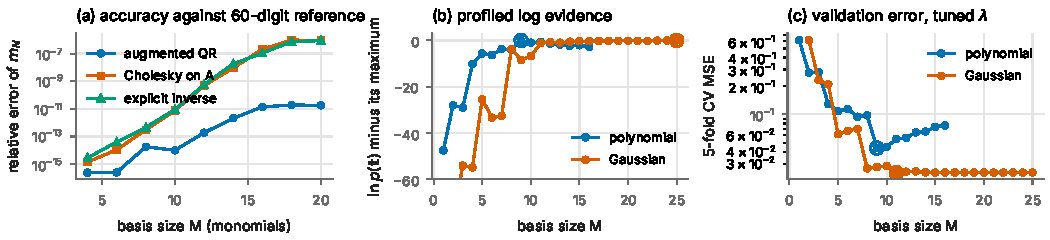
\includegraphics[width=\textwidth]{fig1.pdf}
\caption{Verification and basis comparison. (a) Relative error of the posterior mean for monomials with $\alpha=10^{-8}$. (b) Profiled log evidence relative to its maximum. (c) Five-fold validation error with tuned $\lambda$. Open circles mark the selected $M$.}
\label{fig:one}
\end{figure}

\section{Results}
\subsection{Polynomial and Gaussian bases}
Figure~\ref{fig:one}b shows the evidence rising steeply until the basis can represent the signal and then flattening. For polynomials it peaks at $M=9$ and is 2.8 nats lower at $M=16$. For the Gaussian basis it is within 1.3 nats of its maximum for all $M\ge11$, and on this dataset the maximum falls at the grid edge $M=25$. Underfitted polynomials treat missing signal as noise, so $\hat\beta=1.6$ at $M=1$ and $10$ at $M=6$, against $31.6$ at $M=9$ and a truth of $25$. With fixed $\alpha_0$ and $\beta_0$ the validation error is U-shaped and rises quickly beyond $M=12$ because of boundary oscillation, and tuning $\lambda$ flattens this rise (Figure~\ref{fig:one}c).

\begin{table}[!htbp]
\centering\footnotesize
\caption{Selected models and test error against the noiseless function. Gaussian entries show $M$ and the width $s$ in brackets, and brackets in the last two columns give the interquartile range.}
\label{tab:one}
\begin{tabular}{@{}llccrr@{}}
\toprule
& & \multicolumn{2}{c}{Main dataset} & \multicolumn{2}{c}{30 datasets, median}\\
\cmidrule(lr){3-4}\cmidrule(l){5-6}
Basis & Criterion & $M$ & Test MSE & $M$ & Test MSE\\
\midrule
Polynomial & Evidence & 9 & 0.0184 & 7 [7, 9] & 0.0649 [0.0589, 0.0757] \\
 & CV, fixed $\alpha_0,\beta_0$ & 11 & 0.0237 & 11 [11, 13.75] & 0.0332 [0.0255, 0.0558] \\
 & CV, tuned $\lambda$ & 9 & 0.0150 & 11 [11, 13.75] & 0.0168 [0.0091, 0.0559] \\
\midrule
Gaussian & Evidence & 25 (0.15) & 0.0060 & 8 [8, 11] & 0.0074 [0.0058, 0.0088] \\
 & CV, fixed $\alpha_0,\beta_0$ & 11 (0.15) & 0.0070 & 8 [8, 10] & 0.0089 [0.0058, 0.0123] \\
 & CV, tuned $\lambda$ & 11 (0.15) & 0.0068 & 10 [8, 12] & 0.0086 [0.0061, 0.0102] \\
\\[-1.6ex]
\bottomrule
\end{tabular}
\end{table}

Across the 30 datasets (Table~\ref{tab:one}), evidence chooses smaller polynomials than either validation rule, with median $M=7$ against 11. These polynomials are too small, with test MSE $0.065$ against $0.017$ for tuned validation, so evidence does not isolate the minimal sufficient degree here. For the Gaussian basis the three rules agree more closely, with median $M$ from 8 to 10, and evidence has the lowest median test error ($0.0074$) and is best in 43\% of datasets. The Gaussian basis beats the polynomial in every dataset under evidence and fixed validation and in 87\% under tuned validation. Conditioning favours neither basis at large $M$, since $\kappa=1.6\times10^{5}$ for the polynomial at $M=15$ and $6.6\times10^{12}$ for the Gaussian basis at $M=25$ and $s=0.25$, where neighbouring functions overlap almost completely. At $x=\pm1.5$ the selected polynomial predicts $345$ and $432$, while the Gaussian model returns to its constant term, $-0.09$.

\subsection{Data regimes, sample size and noise}
Figure~\ref{fig:two} and Table~\ref{tab:two} summarise the evidence-selected models. Interpolation error falls with $N$ for every process and basis. For the smooth function the median signal MSE of the Gaussian basis falls from $0.019$ to $0.0052$ to $0.0015$ as $N$ goes from 20 to 60 to 200, against $0.130$, $0.0142$ and $0.0033$ for polynomials. The Gaussian basis has lower interpolation MSE in 83\%, 98\% and 81\% of datasets for the smooth, sharp and heteroscedastic processes. The sharp feature separates the bases most. Polynomials select only $M=3$ to 9 and smooth over the spike or ring across the interval, with MSE $0.097$ at $N=60$, while the Gaussian basis selects a narrow width, $s=0.06$ to $0.12$, and reaches $0.018$.

\begin{figure}[!htbp]
\centering
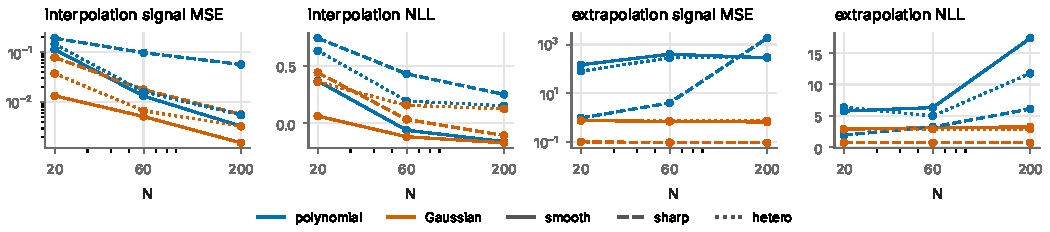
\includegraphics[width=\textwidth]{fig2.pdf}
\caption{Median metrics of evidence-selected models against sample size at $\sigma_0=0.20$, over 30 replicates. Colour shows the basis and line style shows the data process.}
\label{fig:two}
\end{figure}

\begin{table}[!htbp]
\centering\footnotesize
\caption{Median results over 30 replicates at $N=60$ and $\sigma_0=0.20$. Test error is measured on interpolation and extrapolation grids.}
\label{tab:two}
\begin{tabular}{@{}llcrrrr@{}}
\toprule
& & & \multicolumn{2}{c}{Interpolation} & \multicolumn{2}{c}{Extrapolation}\\
\cmidrule(lr){4-5}\cmidrule(l){6-7}
Process & Basis & $M$ & MSE & NLL & MSE & NLL\\
\midrule
smooth & polynomial & 7 & 0.0133 & -0.06 & 400 & 6.31 \\
 & Gaussian & 28 & 0.0052 & -0.12 & 0.686 & 3.09 \\
\midrule
sharp & polynomial & 4 & 0.0971 & 0.43 & 4.01 & 3.21 \\
 & Gaussian & 15 & 0.0179 & 0.03 & 0.0931 & 0.68 \\
\midrule
hetero & polynomial & 7 & 0.0161 & 0.19 & 287 & 4.96 \\
 & Gaussian & 29 & 0.0067 & 0.16 & 0.718 & 2.87 \\
\\[-1.6ex]
\bottomrule
\end{tabular}
\end{table}

Extrapolation shows the reverse of the interpolation trend for polynomials. Their extrapolation MSE grows with $N$ because richer data justify higher degree, rising for the smooth function from 158 to 191 to 296 and for the sharp function from $0.74$ to $3.9$ to $1745$. The Gaussian basis stays flat, near $0.6$ to $0.7$ for the smooth function and $0.09$ for the sharp one, since it reverts to its bias. Its extrapolation NLL is lower in 85\% to 92\% of datasets. Both bases are overconfident outside the data. At $N=60$ and $\sigma_0=0.20$ the 95\% predictive intervals cover $57\%$, $79\%$ and $63\%$ of extrapolation points for the Gaussian basis on the three processes, and only $36\%$, $55\%$ and $43\%$ for polynomials.

A larger noise level selects simpler polynomials, with median $M=9,7,5.5$ for the smooth function at $\sigma_0=0.05,0.20,0.50$. Under input-dependent noise the evidence estimates a single level, $0.264$ on average at $N=200$ and $\sigma_0=0.20$, close to the root mean square of $\sigma(x)$, $0.263$. In a representative dataset the predictive standard deviation is about $0.24$ on both halves, while the true values average $0.098$ on the left and $0.352$ on the right. The 95\% interval covers $100\%$ of the left half and $81\%$ of the right half for polynomials ($99\%$ and $78\%$ for Gaussian), so the model is underconfident where noise is low and overconfident where it is high. Signal MSE is hardly affected, so only the predictive intervals expose this failure.

\subsection{Basis rescaling}
We rescale the two selected bases, the polynomial with $M=9$ and the Gaussian basis with $M=25$ and $s=0.15$, keeping $\alpha$ and $\beta$ at their evidence optimum. Table~\ref{tab:three} shows that keeping the isotropic prior lowers the evidence by 2.3 to 316 nats and moves the extrapolated polynomial mean by up to 365. Re-optimising $\alpha$ and $\beta$ repairs only the uniform scaling, since $c=3$ is absorbed by $\alpha\to\alpha/9$. The decaying scale is the worst case, as it gives the high-order weights small prior variance when this oscillatory target needs them. The growing scale raises the polynomial evidence by 3.2 nats after re-optimisation, so the evidence compares priors as well as bases.

\begin{table}[!htbp]
\centering\footnotesize
\caption{Change in log evidence from the unscaled model when the isotropic prior is kept (naive), after re-optimising $\alpha,\beta$, and the largest change in the extrapolated predictive mean.}
\label{tab:three}
\begin{tabular}{@{}lrrrrrr@{}}
\toprule
& \multicolumn{3}{c}{Polynomial, $M=9$} & \multicolumn{3}{c}{Gaussian, $M=25$}\\
\cmidrule(lr){2-4}\cmidrule(l){5-7}
Scaling & naive & re-opt. & max $|\Delta\mu|$ & naive & re-opt. & max $|\Delta\mu|$\\
\midrule
uniform, $c=3$ & $-5.7$ & $0.0$ & 53 & $-7.2$ & $-0.1$ & 0.0961 \\
decay, $c_m=e^{-0.25m}$ & $-18.7$ & $-5.0$ & 365 & $-316.5$ & $-24.6$ & 0.855 \\
growth, $c_m=e^{0.25m}$ & $-4.6$ & $3.2$ & 56.2 & $-36.5$ & $-17.8$ & 1.41 \\
random, log-normal & $-2.3$ & $-1.7$ & 46.5 & $-6.8$ & $-5.4$ & 0.413 \\
\\[-1.6ex]
\bottomrule
\end{tabular}
\end{table}

With the transformed prior $\tilde\Lambda_0=\alpha C^2$ every quantity matches the original model to rounding error. Over the four scalings the log evidence differs by at most $2.3\times10^{-13}$, the predictive mean by $1.2\times10^{-11}$, the predictive variance by $9.1\times10^{-11}$, and $C\tilde m_N$ equals $m_N$ to $1.6\times10^{-12}$, in line with \eqref{eq:invariance}. A random dense invertible $T$ with precision $\alpha T^\top T$ agrees to $8.5\times10^{-12}$.

\subsection{Systematic disagreement between evidence and validation}
A sparse high-degree monomial cannot be used here, since $x^{11}$ lies within $0.003$ of a degree-9 polynomial on $[-1,1]$ and neither criterion can identify its degree. The orthonormal setting avoids this (Figure~\ref{fig:four}, Table~\ref{tab:four}).

\begin{figure}[!htbp]
\centering
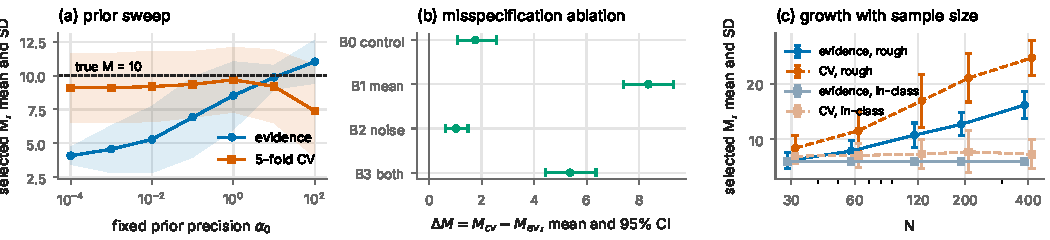
\includegraphics[width=\textwidth]{fig4.pdf}
\caption{Disagreement experiments over 100 datasets per setting. (a) Selected $M$ against fixed prior precision. (b) Paired gap in the misspecification ablation at $N=200$. (c) Selected $M$ against sample size.}
\label{fig:four}
\end{figure}

\textbf{Role of the prior.} In E1 cross-validation hardly reacts to the prior, with mean $M_{\rm cv}$ between 9.1 and 9.7 for $\alpha_0\le1$. The evidence reacts strongly and rises from $M_{\rm ev}=4.1$ at $\alpha_0=10^{-4}$ to $11.0$ at $\alpha_0=100$. The gap $\Delta M$ falls from $+5.0$ to $-3.6$ and changes sign between $\alpha_0=1$ and $10$. Equation \eqref{eq:evidence} explains this. Each well-determined weight costs about $\frac12\ln(1+\beta N/\alpha_0)$ nats, which is $8.6$, $3.9$ and $1.6$ at $\alpha_0=10^{-4}$, $1$ and $100$. Including the degree-9 term needs six extra weights and gains about $\beta N a^2/2\approx30$ nats of log-likelihood, with $a=0.15$ its true weight. The extra cost is $52$ nats for a vague prior but only about $10$ for $\alpha_0=100$. With estimated hyper-parameters evidence selects $M_{\rm ev}=9.4$ and the large gap disappears. At the vague end validation also generalises better (Table~\ref{tab:four}).

\begin{table}[!htbp]
\centering\footnotesize
\caption{Paired comparison over 100 datasets. Mean selected sizes, the gap $\Delta M$ with a 95\% bootstrap interval, the share of datasets with $M_{\rm cv}>M_{\rm ev}$, and median test MSE.}
\label{tab:four}
\begin{tabular}{@{}lcccccc@{}}
\toprule
Setting & $M_{\rm ev}$ & $M_{\rm cv}$ & $\Delta M$ [95\% CI] & $P(M_{\rm cv}>M_{\rm ev})$ & MSE ev. & MSE cv.\\
\midrule
E1, $\alpha_0=10^{-4}$ & 4.1 & 9.1 & $+5.0$ [$+4.5$, $+5.5$] & 0.86 & $2.7\times10^{-2}$ & $7.5\times10^{-3}$ \\
E1, $\alpha_0=100$ & 11.0 & 7.4 & $-3.6$ [$-4.4$, $-2.9$] & 0.11 & $1.4\times10^{-2}$ & $2.8\times10^{-2}$ \\
E1, free hyper-parameters & 9.4 & 10.6 & $+1.2$ [$+0.7$, $+1.7$] & 0.43 & $5.8\times10^{-3}$ & $7.3\times10^{-3}$ \\
\midrule
E2, B0 in-class control & 6.0 & 7.8 & $+1.8$ [$+1.1$, $+2.5$] & 0.36 & $7.2\times10^{-5}$ & $9.4\times10^{-5}$ \\
E2, B1 rough mean & 12.7 & 21.1 & $+8.4$ [$+7.4$, $+9.3$] & 0.97 & $1.0\times10^{-3}$ & $8.2\times10^{-4}$ \\
E2, B2 heavy-tailed noise & 6.0 & 7.1 & $+1.0$ [$+0.6$, $+1.5$] & 0.31 & $6.5\times10^{-4}$ & $8.6\times10^{-4}$ \\
E2, B3 rough mean and heavy tails & 6.5 & 11.9 & $+5.4$ [$+4.5$, $+6.4$] & 0.82 & $4.4\times10^{-3}$ & $3.2\times10^{-3}$ \\
\\[-1.6ex]
\bottomrule
\end{tabular}
\end{table}

\textbf{Role of misspecification.} In E2 the in-class control has a small gap of $+1.8$, because validation scatters upward from the true $M=6$ (standard deviation $3.8$, against $0$ for evidence) and is never lower. Heavy-tailed noise alone gives $+1.0$, no more than the control. A non-polynomial mean gives $+8.4$ with interval $[7.4,9.3]$, and validation chooses the larger model in $97\%$ of datasets. With both, the gap is $+5.4$. The mean, not the noise, drives the disagreement, and the within-method spread, with standard deviation $2.1$ for evidence and $4.3$ for validation, is much smaller than the gap. In E3 the gap for the non-polynomial mean grows from $+2.3$ at $N=30$ to $+8.5$ at $N=400$, while the in-class gap stays between $+1.0$ and $+1.8$. Validation also generalises better under this misspecification, with lower test MSE in 62\% of datasets at $N=200$ and 85\% at $N=400$, whereas evidence does better in class. This is consistent with the evidence being the product of one-step-ahead predictive densities, which averages performance over training sizes from $0$ to $N-1$, while five-fold validation uses $0.8N$ points. When the truth is outside the class the best complexity grows with training size, so the average favours smaller models.

\section{Discussion and limitations}
Neither criterion is better in general. Evidence is sensitive to the prior and rewards parsimony, and it generalised best when the prior suited the data. Validation is insensitive to prior volume and tracks held-out error, so it does better when the model class is wrong, but it is noisier. Since an isotropic prior is not scale free, evidence values are comparable across bases only after normalising columns or using the transformed prior. The limitations are that all data are synthetic with a few noise levels, hyper-parameters are searched on finite grids with one Gaussian optimum on the boundary, Gaussian $M$ is weakly identified because overlapping functions are nearly collinear, each validation result uses one set of folds and squared error only, and Part 5 uses a Legendre basis rather than monomials. The training-size explanation of the gap was not tested directly.

\section{Conclusion}
\begin{enumerate}
\item The augmented QR implementation stays accurate to $2\times10^{-11}$ at condition number $1.5\times10^{7}$, where Cholesky and explicit inversion lose six digits.
\item Evidence-selected polynomials were too small on the benchmark, with test MSE $0.065$ against $0.017$ for tuned validation, and the Gaussian basis beat polynomials in at least 87\% of datasets.
\item Gaussian bases extrapolate with bounded error and polynomials do not, but both are overconfident, and under heteroscedastic noise only interval coverage shows the failure.
\item An isotropic prior is not invariant to basis scaling, and the prior with precision $\alpha C^2$ restores identical posterior, predictions and evidence to about $10^{-13}$.
\item Evidence and validation disagree systematically under a vague fixed prior, with a gap of $+5.0$ basis functions, and under a non-polynomial mean, with $+8.4$ at $N=200$. Heavy-tailed noise alone does not.
\end{enumerate}

\noindent\textbf{Reproducibility.} All numbers, figures and tables are regenerated by \texttt{run\_all.sh} with fixed seeds, and raw per-dataset results are saved as CSV files.

\begin{thebibliography}{9}\footnotesize
\setlength{\itemsep}{0pt}
\bibitem{lm} H. Mukherjee. Linear Models for Regression. Lecture slides, MAC F312, BITS Pilani, K. K. Birla Goa Campus.
\bibitem{gi} H. Mukherjee. Gaussian Inference. Lecture slides, MAC F312, BITS Pilani, K. K. Birla Goa Campus.
\bibitem{g} H. Mukherjee. Multivariate Gaussian Distributions. Lecture slides, MAC F312, BITS Pilani, K. K. Birla Goa Campus.
\end{thebibliography}
\nocite{*}

\end{document}
